\section{Gestion des FAQ}

\begin{center}
\scalebox{0.7}{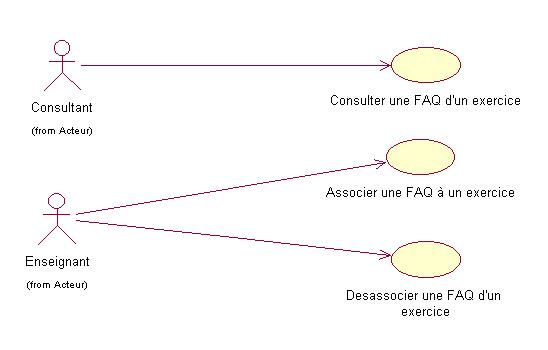
\includegraphics{images/FAQ.jpg}}\\
\par{Package Gestion Faq}
\end{center}
Voici les diff{\'e}rents sc{\'e}narios:\\



\section*{Consultant}

	\begin{tabular}{|p{4cm}|c|p{4cm}|p{5cm}|}
	\hline
	Fonction & Priorit{\'e} & Qualit{\'e} & Mesure \\
	\hline
	Consulter la FAQ d'un exercice & 1 & Lisibilit{\'e} & Bonne distinction entre les questions et les r{\'e}ponses gr{\^a}ce {\`a} l'utilisation de couleurs.\\
	\hline
	\end{tabular}\\

	\begin{center}
	{\'e}chelle de mesure de la priorit{\'e}:

	\scalebox{0.5}{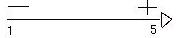
\includegraphics{images/echelle.jpg}}
	\end{center}
	
	\begin{itemize}
	\item {\bf Consulter une FAQ d'un exercice:}
		\begin{itemize}
		\item Pr	{\'e}-requis : Etre log{\'e}/identifi{\'e}.\\
		L'exercice poss{\`e}	de une FAQ.
		\item Description :  L'u	tilisateur s{\'e}lectionne un exercice.\\
		L'utilisateur consulte le fichie	r FAQ associ{\'e} {\`a} l'exercice.
		\item Post-requis : La FAQ de l'exercice	 s{\'e}lectionn{\'e} est affich{\'e}e.
		\end{itemize}			
	\end{itemize}	


\section*{Enseignant}

\begin{tabular}{|p{4cm}|c|p{4cm}|p{5cm}|}
\hline
Fonction & Priorit{\'e} & Qualit{\'e} & Mesure \\
\hline
Associer une FAQ {\`a} un exercice & 1 & Facilit{\'e} & Utilisation de menus simples\\
\hline
D{\'e}sassocier une FAQ {\`a} un exercice & 1 & Facilit{\'e} & Action simple sans archivage\\
\hline
\end{tabular}\\

\begin{center}
{\'e}chelle de mesure de la priorit{\'e}:

\scalebox{0.5}{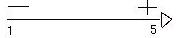
\includegraphics{images/echelle.jpg}}
\end{center}

\begin{itemize}
\item {\bf Associer une FAQ {\`a} un exercice:}
	\begin{itemize}
	\item Pr{\'e}-requis : Etre log{\'e}/identifi{\'e}.\\
	L'exercice ne poss{\`e}de pas encore de FAQ.
	\item Description :  L'utilisateur selectionne un exercice.\\
	L'utilisateur clique l'option {\it Ajouter une FAQ}.\\
	L'utilisateur choisit un fichier qui se trouve sur son compte.
	L'utilisateur importe un fichier FAQ et l'associe {\`a} cet exercice.
	\item Post-requis : L'exercice poss{\`e}de une FAQ associ{\'e}e.
	\end{itemize}

\item {\bf D{\'e}sassocier une FAQ d'un exercice:}
	\begin{itemize}
	\item Pr{\'e}-requis : Etre log{\'e}/identifi{\'e}.\\
	L'exercice poss{\`e}de une FAQ.
	\item Description :  L'utilisateur selectionne un exercice.\\
	L'utilisateur clique sur l'option {\it Supprimer une FAQ}.
	\item Post-requis : L'exercice ne poss{\`e}de plus de FAQ associ{\'e}e.\\
	\end{itemize}
\end{itemize}


